\documentclass[a4paper, 10pt]{article}
\usepackage[utf8]{inputenc}
\usepackage[T1]{fontenc}
\usepackage{geometry}
\usepackage{amsmath, amssymb, xcolor} % Aggiunto xcolor per sicurezza
\usepackage{pgfplots}
\usepackage{multicol}
\usepackage{enumitem}

% Impostazioni pagina: Margini stretti
\geometry{top=1cm, bottom=1cm, left=1cm, right=1cm}
\pgfplotsset{compat=1.18}

% Stile standard per i grafici
\pgfplotsset{
    standard/.style={
        axis lines=middle,
        xlabel=$x$, ylabel=$y$,
        width=7.5cm, height=4.5cm, % Leggermente più larghi
        tick label style={font=\tiny},
        label style={font=\small},
        grid=both,
        grid style={line width=.1pt, draw=gray!20},
        every axis x label/.style={at={(current axis.right of origin)},anchor=north west},
        every axis y label/.style={at={(current axis.above origin)},anchor=south east}
    }
}

% Comando per bloccare insieme Titolo + Grafico + Descrizione
\newcommand{\block}[1]{
    \noindent
    \begin{minipage}{\linewidth}
        #1
    \end{minipage}
    \vspace{0.4cm} % Spazio tra un blocco e l'altro
}

\title{\vspace{-2cm}\textbf{Formulario Grafici e Funzioni}}
\date{}
\author{}

\begin{document}
{\centering \large \textbf{Formulario Analisi 1: Grafici Fondamentali} \par}
\vspace{0.3cm}

\begin{multicols}{2}

% --- POTENZE ---
\section*{1. Potenze e Razionali}

\block{
    \textbf{Parabola: $y = x^2$} (Pari)
    \begin{center}
    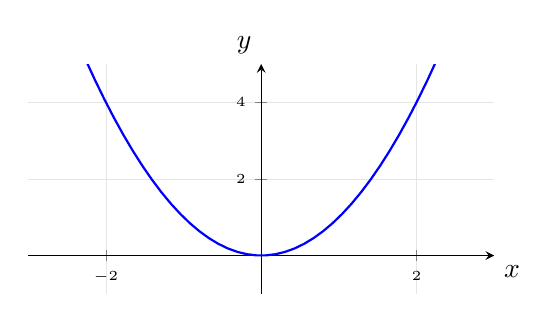
\begin{tikzpicture}
    \begin{axis}[standard, ymin=-1, ymax=5, xmin=-3, xmax=3]
        \addplot[thick, blue, domain=-3:3, samples=50] {x^2};
    \end{axis}
    \end{tikzpicture}
    \end{center}
    \footnotesize $D: \mathbb{R}$, $Im: [0, +\infty)$. Convessa $\cup$.
}

\block{
    \textbf{Iperbole Equilatera: $y = 1/x$} (Dispari)
    \begin{center}
    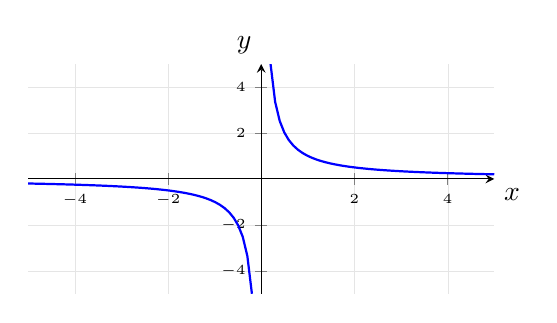
\begin{tikzpicture}
    \begin{axis}[standard, ymin=-5, ymax=5, xmin=-5, xmax=5]
        \addplot[thick, blue, domain=-5:-0.2, samples=50] {1/x};
        \addplot[thick, blue, domain=0.2:5, samples=50] {1/x};
    \end{axis}
    \end{tikzpicture}
    \end{center}
    \footnotesize $D: \mathbb{R} \setminus \{0\}$. Asintoti: $x=0, y=0$.
}

\block{
    \textbf{Radice Quadrata: $y = \sqrt{x}$}
    \begin{center}
    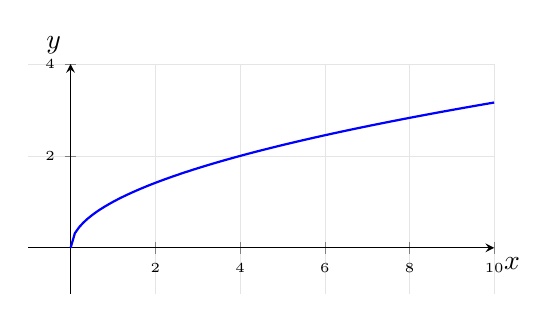
\begin{tikzpicture}
    \begin{axis}[standard, ymin=-1, ymax=4, xmin=-1, xmax=10]
        \addplot[thick, blue, domain=0:10, samples=100] {sqrt(x)};
    \end{axis}
    \end{tikzpicture}
    \end{center}
    \footnotesize $D: [0, +\infty)$. Derivata verticale in $0$.
}

% --- NUOVA SEZIONE POLINOMI ---
\section*{2. Polinomi (Comportamento)}

\block{
    \textbf{Grado DISPARI ($x^3, x^5...$)} \\
    \textit{Uno su, uno giù.}
    \begin{center}
    \begin{tabular}{c c}
        \textbf{ coeff $> 0$} & \textbf{coeff $< 0$} \\
        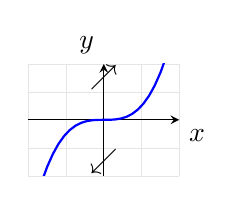
\begin{tikzpicture}[baseline]
            \begin{axis}[standard, width=3.5cm, height=3cm, ymin=-4, ymax=4, xmin=-2, xmax=2, ticks=none]
                \addplot[thick, blue, domain=-1.8:1.8] {x^3};
                \node at (axis cs:0,3) {$\nearrow$}; \node at (axis cs:0,-3) {$\swarrow$};
            \end{axis}
        \end{tikzpicture} 
        & 
        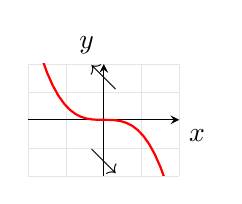
\begin{tikzpicture}[baseline]
            \begin{axis}[standard, width=3.5cm, height=3cm, ymin=-4, ymax=4, xmin=-2, xmax=2, ticks=none]
                \addplot[thick, red, domain=-1.8:1.8] {-x^3};
                \node at (axis cs:0,3) {$\nwarrow$}; \node at (axis cs:0,-3) {$\searrow$};
            \end{axis}
        \end{tikzpicture}
    \end{tabular}
    \end{center}
}

\block{
    \textbf{Grado PARI ($x^4, x^6...$)} \\
    \textit{Entrambi stessa direzione.}
    \begin{center}
    \begin{tabular}{c c}
        \textbf{ coeff $> 0$} & \textbf{coeff $< 0$} \\
        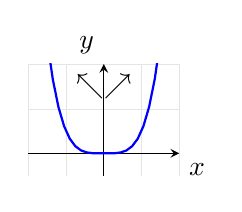
\begin{tikzpicture}[baseline]
            \begin{axis}[standard, width=3.5cm, height=3cm, ymin=-1, ymax=4, xmin=-2, xmax=2, ticks=none]
                \addplot[thick, blue, domain=-1.8:1.8] {x^4};
                \node at (axis cs:0,3) {$\nwarrow \nearrow$};
            \end{axis}
        \end{tikzpicture} 
        & 
        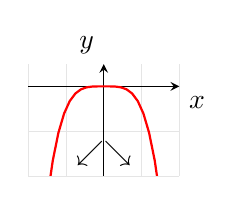
\begin{tikzpicture}[baseline]
            \begin{axis}[standard, width=3.5cm, height=3cm, ymin=-4, ymax=1, xmin=-2, xmax=2, ticks=none]
                \addplot[thick, red, domain=-1.8:1.8] {-x^4};
                \node at (axis cs:0,-3) {$\swarrow \searrow$};
            \end{axis}
        \end{tikzpicture}
    \end{tabular}
    \end{center}
}

% --- EXP & LOG ---
\section*{3. Esponenziali e Logaritmi}

\block{
    \textbf{Esponenziale: $y = e^x$}
    \begin{center}
    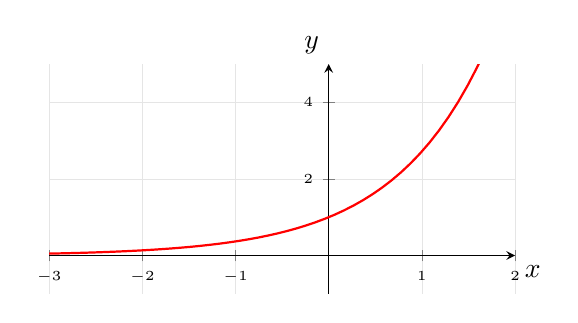
\begin{tikzpicture}
    \begin{axis}[standard, ymin=-1, ymax=5, xmin=-3, xmax=2]
        \addplot[thick, red, domain=-3:2, samples=50] {exp(x)};
    \end{axis}
    \end{tikzpicture}
    \end{center}
    \footnotesize $Im: (0, +\infty)$. Cresce velocissima.
}

\block{
    \textbf{Logaritmo: $y = \ln(x)$}
    \begin{center}
    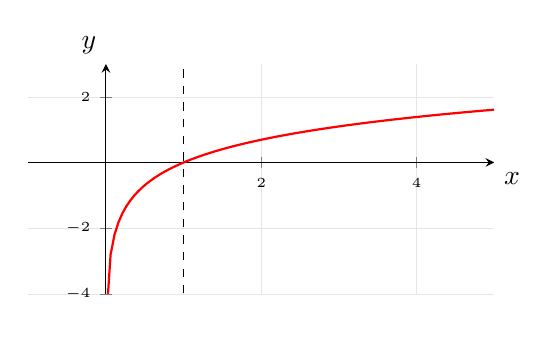
\begin{tikzpicture}
    \begin{axis}[standard, ymin=-4, ymax=3, xmin=-1, xmax=5]
        \addplot[thick, red, domain=0.01:5, samples=100] {ln(x)};
        \draw[dashed] (axis cs:1,-5) -- (axis cs:1,5);
    \end{axis}
    \end{tikzpicture}
    \end{center}
    \footnotesize $D: (0, +\infty)$. Asintoto vert: $x=0$.
}

% --- COLONNA 2 ---
\columnbreak 

% --- VALORE ASSOLUTO ---
\section*{4. Valore Assoluto}

\block{
    \textbf{$y = |x|$} (Pari)
    \begin{center}
    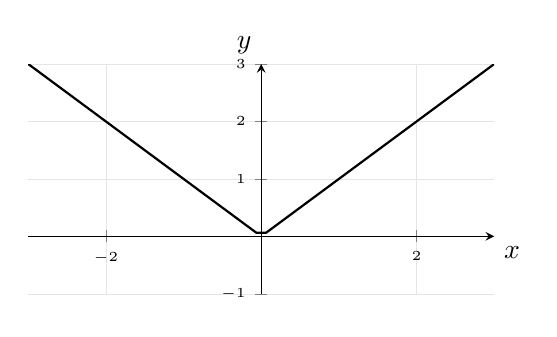
\begin{tikzpicture}
    \begin{axis}[standard, ymin=-1, ymax=3, xmin=-3, xmax=3]
        \addplot[thick, black, domain=-3:3, samples=50] {abs(x)};
    \end{axis}
    \end{tikzpicture}
    \end{center}
    \footnotesize $f(x) = x$ se $x \ge 0$, $-x$ se $x < 0$.
    \textbf{Non derivabile} in $x=0$ (Punto angoloso).
}

% --- TRIGONOMETRIA ---
\section*{5. Trigonometria}

\block{
    \textbf{Seno e Coseno}
    \begin{center}
    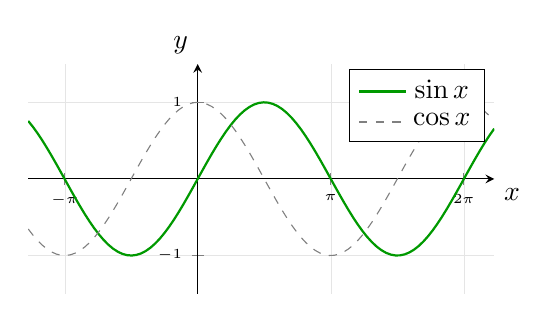
\begin{tikzpicture}
    \begin{axis}[standard, ymin=-1.5, ymax=1.5, xmin=-4, xmax=7, xtick={-3.14, 0, 3.14, 6.28}, xticklabels={$-\pi$, $0$, $\pi$, $2\pi$}]
        \addplot[thick, green!60!black, domain=-4:7, samples=100] {sin(deg(x))};
        \addplot[dashed, gray, domain=-4:7, samples=100] {cos(deg(x))};
        \legend{$\sin x$, $\cos x$}
    \end{axis}
    \end{tikzpicture}
    \end{center}
    \footnotesize Periodo $2\pi$. Sin dispari, Cos pari.
}

\block{
    \textbf{Tangente: $y = \tan(x)$}
    \begin{center}
    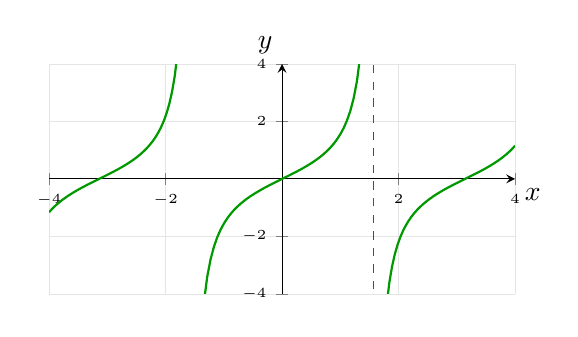
\begin{tikzpicture}
    \begin{axis}[standard, ymin=-4, ymax=4, xmin=-4, xmax=4, restrict y to domain=-5:5]
        \addplot[thick, green!60!black, domain=-1.4:1.4, samples=50] {tan(deg(x))};
        \addplot[thick, green!60!black, domain=1.7:4, samples=50] {tan(deg(x))};
        \addplot[thick, green!60!black, domain=-4:-1.7, samples=50] {tan(deg(x))};
        \draw[dashed, red] (axis cs:1.57,-5) -- (axis cs:1.57,5);
    \end{axis}
    \end{tikzpicture}
    \end{center}
    \footnotesize Asintoti vert: $\pm \frac{\pi}{2}$. Periodo $\pi$.
}

% --- INVERSE ---
\section*{6. Inverse (Fondamentali)}

\block{
    \textbf{Arcotangente: $y = \arctan(x)$} \textcolor{red}{(!)}
    \begin{center}
    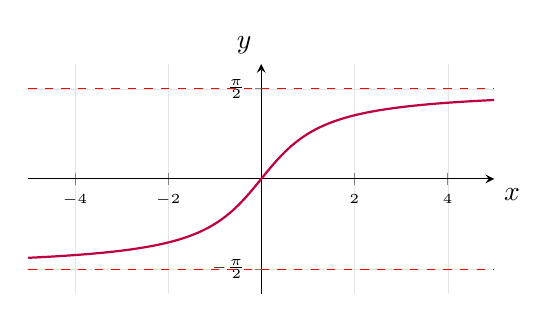
\begin{tikzpicture}
    \begin{axis}[standard, ymin=-2, ymax=2, xmin=-5, xmax=5, ytick={-1.57, 0, 1.57}, yticklabels={$-\frac{\pi}{2}$, $0$, $\frac{\pi}{2}$}]
        \addplot[thick, purple, domain=-5:5, samples=100] {rad(atan(x))};
        \draw[dashed, red] (axis cs:-5,1.57) -- (axis cs:5,1.57);
        \draw[dashed, red] (axis cs:-5,-1.57) -- (axis cs:5,-1.57);
    \end{axis}
    \end{tikzpicture}
    \end{center}
    \footnotesize $D: \mathbb{R}$. Asintoti Orizz: $y = \pm \frac{\pi}{2}$.
}

\block{
    \textbf{Arcoseno: $y = \arcsin(x)$}
    \begin{center}
    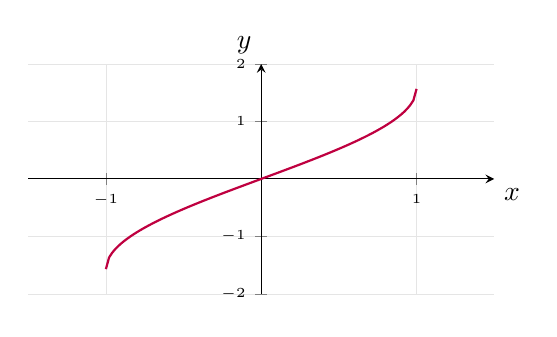
\begin{tikzpicture}
    \begin{axis}[standard, ymin=-2, ymax=2, xmin=-1.5, xmax=1.5]
        \addplot[thick, purple, domain=-1:1, samples=100] {rad(asin(x))};
    \end{axis}
    \end{tikzpicture}
    \end{center}
    \footnotesize $D: [-1, 1]$. Tangenti verticali agli estremi.
}
% --- IPERBOLICHE ---
\section*{6. Funzioni Iperboliche}

\block{
    \textbf{Seno Iperbolico: $\sinh(x)$} (Dispari)
    \begin{center}
    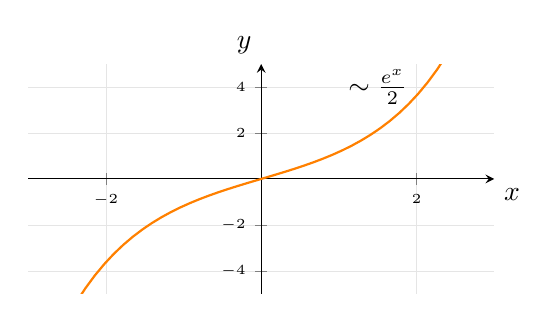
\begin{tikzpicture}
    \begin{axis}[standard, ymin=-5, ymax=5, xmin=-3, xmax=3]
        \addplot[thick, orange, domain=-3:3, samples=50] {sinh(x)};
        \node at (axis cs:1.5,4) {$\sim \frac{e^x}{2}$};
    \end{axis}
    \end{tikzpicture}
    \end{center}
    \footnotesize Def: $\dfrac{e^x - e^{-x}}{2}$. Simile a $x^3$. $D: \mathbb{R}$.
}

\block{
    \textbf{Coseno Iperbolico: $\cosh(x)$} (Pari)
    \begin{center}
    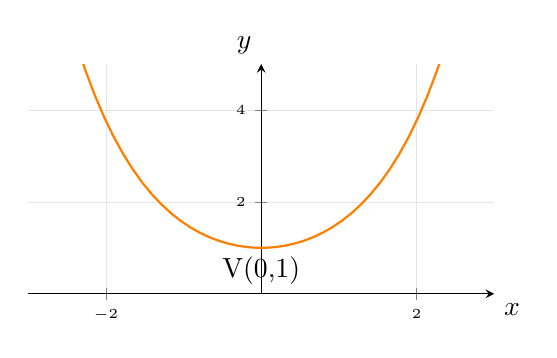
\begin{tikzpicture}
    \begin{axis}[standard, ymin=0, ymax=5, xmin=-3, xmax=3]
        \addplot[thick, orange, domain=-3:3, samples=50] {cosh(x)};
        \node at (axis cs:0,0.5) {V(0,1)};
    \end{axis}
    \end{tikzpicture}
    \end{center}
    \footnotesize Def: $\dfrac{e^x + e^{-x}}{2}$. Simile a $x^2$. $Im: [1, +\infty)$.
}

\block{
    \textbf{Le 2 Formule "Salva-Vita"} \\
    \textit{Da usare per semplificare equazioni e limiti.}
    
    \textbf{1. Relazione Fondamentale (Iperbole)}
    \[ \cosh^2(x) - \sinh^2(x) = 1 \]
    \textit{Nota il MENO! (nella trigonometria normale è +)}
    
    \textbf{2. Regola delle Derivate}
    \begin{itemize}
        \item $D[\sinh x] = \cosh x$
        \item $D[\cosh x] = \sinh x$ \quad \textcolor{red}{(Niente meno!)}
    \end{itemize}
}
\end{multicols}


\newpage
 \section*{11. Forme Indeterminate e Strategie}

\block{
    \textbf{Le 7 Forme Indeterminate} \\
    \textit{Se ottieni una di queste, il limite non è finito: devi lavorarci.}
    
    \renewcommand{\arraystretch}{1.6}
    \begin{center}
    \begin{tabular}{|p{2.5cm}|p{2.5cm}|p{6cm}|}
        \hline
        \textbf{Tipo} & \textbf{Forma} & \textbf{Strategia / Trucco} \\ \hline
        
        \textbf{Algebriche}
        & $\infty - \infty$ 
        & Raccogli la potenza più alta ("il più forte") o Razionalizza (se ci sono radici). \\ \hline
        
        \textbf{Algebriche}
        & $0 \cdot \infty$ 
        & Trasforma in frazione: $f \cdot g = \frac{f}{1/g}$. Diventerà $0/0$ o $\infty/\infty$. \\ \hline
        
        \textbf{Algebriche}
        & $\dfrac{0}{0}$ 
        & Usare Sviluppi di Taylor (consigliato per funzioni miste) o De L'Hôpital. \\ \hline
        
        \textbf{Algebriche}
        & $\dfrac{\infty}{\infty}$ 
        & Vince la gerarchia degli infiniti (vedi sotto) o De L'Hôpital. \\ \hline
        
        \textbf{Esponenziali}
        & $1^{\infty}, \ 0^0, \ \infty^0$
        & Usa la trasformazione fondamentale: \newline 
        $f(x)^{g(x)} = e^{g(x) \cdot \ln(f(x))}$ \newline 
        Poi calcola il limite dell'esponente. \\ \hline
    \end{tabular}
    \end{center}
    \renewcommand{\arraystretch}{1}
}

\block{
    \textbf{Gerarchia degli Infiniti ($x \to +\infty$)} \\
    \textit{Chi "vince" determina il risultato. Ordine dal più lento al più veloce:}
    
    \[ \ln x \ll x^a \ll a^x \ll x! \ll x^x \]
    
    \begin{itemize}
        \item $\ln x$: Perde sempre (va a infinito lentissimo).
        \item $x^n$: Le potenze perdono contro gli esponenziali.
        \item $e^x$: Vince contro qualsiasi polinomio.
    \end{itemize}
}

\block{
    \textbf{Attenzione: NON sono Indeterminate} \\
    \textit{Questi fanno subito il risultato scritto, non applicare L'Hôpital!}
    
    \begin{itemize}
        \item $\dfrac{0}{\infty} = 0$ \quad (Zero diviso qualsiasi cosa fa zero)
        \item $\dfrac{\infty}{0} = \infty$ \quad (Enorme diviso piccolissimo fa enorme)
        \item $+\infty + \infty = +\infty$
        \item $0^{+\infty} = 0$
    \end{itemize}
}
\section*{7. Equivalenze Asintotiche e Limiti Notevoli}

\block{
    \textbf{Sviluppi Fondamentali per $x \to 0$} \\
    \textit{Valgono se l'argomento tende a 0 (anche se è una funzione $f(x) \to 0$).}
    
    \renewcommand{\arraystretch}{1.5} % Spazia meglio le righe
    \begin{center}
    \begin{tabular}{|l|l|}
        \hline
        \textbf{Funzione} & \textbf{Equivalente ($x \to 0$)} \\ \hline
        $\sin(x)$ & $\sim x$ \\ \hline
        $\tan(x)$ & $\sim x$ \\ \hline
        $\arcsin(x)$ & $\sim x$ \\ \hline
        $\arctan(x)$ & $\sim x$ \\ \hline
        $1 - \cos(x)$ & $\sim \frac{1}{2}x^2$ \quad \textcolor{red}{(!)} \\ \hline
        $e^x - 1$ & $\sim x$ \\ \hline
        $\ln(1+x)$ & $\sim x$ \\ \hline
        $(1+x)^\alpha - 1$ & $\sim \alpha x$ \\ \hline
        $\sinh(x)$ & $\sim x$ \\ \hline
        $\cosh(x) - 1$ & $\sim \frac{1}{2}x^2$ \\ \hline
    \end{tabular}
    \end{center}
    \footnotesize \textbf{Esempio:} $\lim_{x\to 0} \frac{\sin(3x)}{x} = \frac{3x}{x} = 3$.
}
\section*{10. Sviluppi di Taylor e Formule Utili}
Se sviluppi centrato in un punto $x_0$ (Taylor):
    \[ f(x) = f(x_0) + f'(x_0)(x-x_0) + \frac{f''(x_0)}{2}(x-x_0)^2 + \frac{f'''(x_0)}{6}(x-x_0)^3 + o((x-x_0)^3) \]
\block{
    \textbf{Sviluppi di McLaurin ($x \to 0$, ordine 3)} \\
    \textit{Tutti gli sviluppi includono $+ o(x^3)$.}
    
    \renewcommand{\arraystretch}{2.2} % Spaziatura per frazioni leggibili
    \begin{center}
    \begin{tabular}{|l|l|}
        \hline
        \textbf{Funzione} & \textbf{Sviluppo} \\ \hline
        
        $e^x$ 
        & $1 + x + \dfrac{x^2}{2} + \dfrac{x^3}{6}$ \\ \hline
        
        $e^{-x}$ 
        & $1 - x + \dfrac{x^2}{2} - \dfrac{x^3}{6}$ \\ \hline
        
        $\ln(1+x)$ 
        & $x - \dfrac{x^2}{2} + \dfrac{x^3}{3}$ \\ \hline
        
        $\sin(x)$ 
        & $x - \dfrac{x^3}{6}$ \\ \hline
        
        $\cos(x)$ 
        & $1 - \dfrac{x^2}{2}$ \quad \footnotesize{(term. $x^3$ nullo)} \\ \hline
        
        $\tan(x)$ 
        & $x + \dfrac{x^3}{3}$ \\ \hline
        
        $\arcsin(x)$ 
        & $x + \dfrac{x^3}{6}$ \\ \hline

        $\arccos(x)$ 
        & $\dfrac{\pi}{2} - x - \dfrac{x^3}{6}$ \\ \hline
        
        $\arctan(x)$ 
        & $x - \dfrac{x^3}{3}$ \\ \hline
        
        $\sinh(x)$ 
        & $x + \dfrac{x^3}{6}$ \\ \hline

        $\sqrt{1+x}$ 
        & $1 + \dfrac{1}{2}x - \dfrac{1}{8}x^2 + \dfrac{1}{16}x^3$ \\ \hline
        
        $(1+x)^\alpha$ 
        & $1 + \alpha x + \dfrac{\alpha(\alpha-1)}{2}x^2 + \dots$ \\ \hline
    \end{tabular}
    \end{center}
    \renewcommand{\arraystretch}{1}
}

\block{
    \textbf{Formule di Addizione (per cambi variabile)} \\
    Utili quando $x \to x_0$ invece di $x \to 0$.
    \begin{itemize}
        \item $\sin(x + a) = \sin x \cos a + \cos x \sin a$
        \item $\cos(x + a) = \cos x \cos a - \sin x \sin a$
    \end{itemize}
}

\section*{11. Trucchi "Salva-Vita" (Cambio Variabile)}

\block{
    \textbf{Come applicare Taylor se l'argomento non è 0?} \\
    \textit{Regola Ferrea: Puoi sostituire $f(t) \sim t$ solo se $t \to 0$.}
    
    \vspace{0.2cm}
    \textbf{1. Il Trucco del "$+1 -1$" (Per Logaritmi)} \\
    Usalo quando hai $\ln(\text{qualcosa})$ e quel "qualcosa" tende a $1$ invece che a $0$.
    Devi ricreare la forma $\ln(1 + \text{mostro})$.
    
    \textbf{Esempio classico ($x \to 1$):}
    \[ \ln(x) = \ln(1 + \underbrace{x - 1}_{t}) \sim x - 1 \]
    
    \textbf{Esempio avanzato ($\ln(\cos x)$ per $x \to 0$):}
    Il coseno tende a 1. Aggiungi e togli 1:
    \[ \ln(\cos x) = \ln(1 + \underbrace{\cos x - 1}_{t}) \sim (\cos x - 1) \sim -\frac{x^2}{2} \]
    
    \vspace{0.2cm}
    \textbf{2. Raccoglimento Forzato (Per costanti diverse da 1)} \\
    Se hai $\ln(2+x)$ o $\sqrt{4+x}$, devi far uscire il numero per ottenere un "1".
    
    \textbf{Esempio Logaritmo:}
    \[ \ln(2+x) = \ln\left[ 2 \left( 1 + \frac{x}{2} \right) \right] = \ln 2 + \ln\left(1+\frac{x}{2}\right) \]
    Ora puoi sviluppare il secondo pezzo ($\sim x/2$).
    
    \textbf{Esempio Radice:}
    \[ \sqrt{4+x} = \sqrt{4 \left( 1 + \frac{x}{4} \right)} = 2 \sqrt{1+\frac{x}{4}} \sim 2 \left(1 + \frac{1}{2}\frac{x}{4}\right) \]
    
    \vspace{0.2cm}
    \textbf{3. Cambio di Variabile Standard ($x \to c$)} \\
    Se il limite non è a 0, poni $t = x - c$ (quindi $t \to 0$).
    Sostituisci $x = c + t$.
    
    \textbf{Esempio ($x \to 2$):}
    \[ e^x \to e^{2+t} = e^2 \cdot e^t \sim e^2 (1+t + \dots) \]
}

\newpage
\section*{13. Tavola delle Derivate Completa}

\block{
    \textbf{A. Derivate Elementari (Da sapere a memoria)}
    
    \renewcommand{\arraystretch}{2.1}
    \begin{center}
    \begin{tabular}{|c|c||c|c|}
        \hline
        $f(x)$ & $f'(x)$ & $f(x)$ & $f'(x)$ \\ \hline
        
        $x^n$ & $n x^{n-1}$ & $\sin x$ & $\cos x$ \\ \hline
        
        $\sqrt{x}$ & $\dfrac{1}{2\sqrt{x}}$ & $\cos x$ & $\textcolor{red}{-}\sin x$ \\ \hline
        
        $\dfrac{1}{x}$ & $-\dfrac{1}{x^2}$ & $\tan x$ & $1+\tan^2 x = \dfrac{1}{\cos^2 x}$ \\ \hline
        
        $e^x$ & $e^x$ & $\arcsin x$ & $\dfrac{1}{\sqrt{1-x^2}}$ \\ \hline
        
        $\ln x$ & $\dfrac{1}{x}$ & $\arccos x$ & $\textcolor{red}{-}\dfrac{1}{\sqrt{1-x^2}}$ \\ \hline
        
        $a^x$ & $a^x \ln a$ & $\arctan x$ & $\dfrac{1}{1+x^2}$ \textcolor{red}{(!)} \\ \hline
        
        $\log_a x$ & $\dfrac{1}{x \ln a}$ & $\sinh x$ & $\cosh x$ \\ \hline
        
        $|x|$ & $\dfrac{x}{|x|} = \text{sgn}(x)$ & $\cosh x$ & $\sinh x$ \\ \hline
    \end{tabular}
    \end{center}
    \renewcommand{\arraystretch}{1}
    
    \textbf{Nota bene su $a^x$ e $\log_a x$:}
    \begin{itemize}
        \item Quando derivi l'esponenziale ($a^x$), il $\ln a$ va al \textbf{numeratore} (moltiplica).
        \item Quando derivi il logaritmo ($\log_a x$), il $\ln a$ va al \textbf{denominatore} (divide).
    \end{itemize}
}

\block{
    \textbf{B. I "Pattern" Ricorrenti (Funzioni Composte)} \\
    \textit{Le strutture che trovi sempre negli esercizi.}
    
    \renewcommand{\arraystretch}{2.2}
    \begin{center}
    \begin{tabular}{|l|l|l|}
        \hline
        \textbf{Tipo} & \textbf{Funzione} & \textbf{Derivata Veloce} \\ \hline
        
        \textbf{Logaritmo} 
        & $\ln(f(x))$ 
        & $\dfrac{f'(x)}{f(x)}$ \\ \hline
        
        \textbf{Radice} 
        & $\sqrt{f(x)}$ 
        & $\dfrac{f'(x)}{2\sqrt{f(x)}}$ \\ \hline
        
        \textbf{Reciproco} 
        & $\dfrac{1}{f(x)}$ 
        & $-\dfrac{f'(x)}{[f(x)]^2}$ \\ \hline
        
        \textbf{Potenza Funz.} 
        & $[f(x)]^n$ 
        & $n [f(x)]^{n-1} \cdot f'(x)$ \\ \hline
        
        \textbf{Esponenziale} 
        & $e^{f(x)}$ 
        & $e^{f(x)} \cdot f'(x)$ \\ \hline
        
        \textbf{Arcotangente} 
        & $\arctan(f(x))$ 
        & $\dfrac{f'(x)}{1 + [f(x)]^2}$ \\ \hline
    \end{tabular}
    \end{center}
    \renewcommand{\arraystretch}{1}
}

\block{
    \textbf{B. I "Pattern" Ricorrenti (Velocizza i calcoli!)} \\
    \textit{Queste sono le derivate composte che escono sempre negli studi di funzione. Impara direttamente la forma finale.}
    
    \renewcommand{\arraystretch}{2.2}
    \begin{center}
    \begin{tabular}{|l|l|l|}
        \hline
        \textbf{Tipo} & \textbf{Funzione} & \textbf{Derivata Veloce} \\ \hline
        
        \textbf{Logaritmo} 
        & $\ln(f(x))$ 
        & $\dfrac{f'(x)}{f(x)}$ \\ \hline
        
        \textbf{Radice} 
        & $\sqrt{f(x)}$ 
        & $\dfrac{f'(x)}{2\sqrt{f(x)}}$ \\ \hline
        
        \textbf{Reciproco} 
        & $\dfrac{1}{f(x)}$ 
        & $-\dfrac{f'(x)}{[f(x)]^2}$ \\ \hline
        
        \textbf{Potenza Funz.} 
        & $[f(x)]^n$ 
        & $n [f(x)]^{n-1} \cdot f'(x)$ \\ \hline
        
        \textbf{Esponenziale} 
        & $e^{f(x)}$ 
        & $e^{f(x)} \cdot f'(x)$ \\ \hline
        
        \textbf{Arcotangente} 
        & $\arctan(f(x))$ 
        & $\dfrac{f'(x)}{1 + [f(x)]^2}$ \\ \hline
    \end{tabular}
    \end{center}
    \renewcommand{\arraystretch}{1}
}

\block{
    \textbf{C. Il "Mostro": Funzione elevata a Funzione} \\
    \[ y = f(x)^{g(x)} \]
    Non usare regole a caso! Usa il trucco dell'esponenziale:
    \[ f(x)^{g(x)} = e^{g(x) \cdot \ln(f(x))} \]
    
    \textbf{Formula finale:}
    \[ D\left[ f(x)^{g(x)} \right] = f(x)^{g(x)} \left[ g'(x)\ln f(x) + g(x)\frac{f'(x)}{f(x)} \right] \]
    \textit{Consiglio: Non imparare la formula a memoria, impara il trucco di scriverlo come $e^{\dots}$ e derivare quello.}
}

\block{
    \textbf{D. Regole di Derivazione (Generali)}
    \begin{itemize}
        \item \textbf{Prodotto:} $(f \cdot g)' = f' g + f g'$
        \item \textbf{Quoziente:} $\left(\dfrac{f}{g}\right)' = \dfrac{f' g - f g'}{g^2}$ \quad \textcolor{red}{(Occhio al meno!)}
        \item \textbf{Catena:} $f(g(x))' = f'(g(x)) \cdot g'(x)$
    \end{itemize}
}
\section*{14. Trigonometria: I Fondamentali}

\block{
    \textbf{1. Tabella dei Valori Noti} \\
    \textit{Questi numeri devono essere automatici.}
    
    \renewcommand{\arraystretch}{1.5}
    \begin{center}
    \begin{tabular}{|c|c||c|c|c|}
        \hline
        \textbf{Rad} & \textbf{Deg} & $\boldsymbol{\sin \alpha}$ & $\boldsymbol{\cos \alpha}$ & $\boldsymbol{\tan \alpha}$ \\ \hline
        $0$ & $0^\circ$ & $0$ & $1$ & $0$ \\ \hline
        $\frac{\pi}{6}$ & $30^\circ$ & $\frac{1}{2}$ & $\frac{\sqrt{3}}{2}$ & $\frac{\sqrt{3}}{3}$ \\ \hline
        $\frac{\pi}{4}$ & $45^\circ$ & $\frac{\sqrt{2}}{2}$ & $\frac{\sqrt{2}}{2}$ & $1$ \\ \hline
        $\frac{\pi}{3}$ & $60^\circ$ & $\frac{\sqrt{3}}{2}$ & $\frac{1}{2}$ & $\sqrt{3}$ \\ \hline
        $\frac{\pi}{2}$ & $90^\circ$ & $1$ & $0$ & $\nexists$ \\ \hline
        $\pi$ & $180^\circ$ & $0$ & $-1$ & $0$ \\ \hline
    \end{tabular}
    \end{center}
    \renewcommand{\arraystretch}{1}
}

\block{
    \textbf{2. Formule di Addizione e Sottrazione}
    \begin{itemize}
        \item $\sin(\alpha \pm \beta) = \sin \alpha \cos \beta \pm \cos \alpha \sin \beta$
        \item $\cos(\alpha \pm \beta) = \cos \alpha \cos \beta \mp \sin \alpha \sin \beta$ \textcolor{red}{(!)}
    \end{itemize}
    \footnotesize \textit{Occhio al coseno: se c'è $+$, nella formula diventa $-$.}
}

\block{
    \textbf{3. Formule di Duplicazione (Cruciali)} \\
    \textit{Servono sempre per semplificare le derivate.}
    
    \textbf{Seno:}
    \[ \sin(2x) = 2 \sin x \cos x \]
    
    \textbf{Coseno (3 versioni):}
    \begin{align*}
        \cos(2x) &= \cos^2 x - \sin^2 x \\
                 &= 2\cos^2 x - 1 \\
                 &= 1 - 2\sin^2 x
    \end{align*}
}

\block{
    \textbf{4. Formule di Bisezione / Linearizzazione} \\
    \textit{VITALI per fare gli integrali di $\sin^2$ e $\cos^2$!}
    
    Invece di usare le radici, impara queste (Linearizzazione):
    \[ \sin^2 x = \frac{1 - \cos(2x)}{2} \]
    \[ \cos^2 x = \frac{1 + \cos(2x)}{2} \]
    \footnotesize Ti permettono di integrare quadrati trasformandoli in coseni semplici.
}

\block{
    \textbf{5. Angoli Associati (Simmetrie)} \\
    \textit{Come ricondursi al primo quadrante.}
    
    \textbf{A. Opposti ($-x$)}:
    \begin{itemize}
        \item $\sin(-x) = -\sin x$ (Dispari)
        \item $\cos(-x) = \cos x$ (Pari, "mangia il meno")
    \end{itemize}
    
    \textbf{B. Supplementari ($\pi - x$)} \textit{(II quadrante)}:
    \begin{itemize}
        \item $\sin(\pi - x) = \sin x$ (Seno uguale)
        \item $\cos(\pi - x) = -\cos x$ (Coseno opposto)
    \end{itemize}
    
    \textbf{C. Complementari ($\frac{\pi}{2} - x$)}:
    \begin{itemize}
        \item $\sin(\frac{\pi}{2}-x) = \cos x$ (Scambio!)
        \item $\cos(\frac{\pi}{2}-x) = \sin x$
    \end{itemize}
}

\block{
    \textbf{6. Relazioni sui Triangoli Rettangoli} \\
    \textit{Risoluzione dei cateti.}
    
    \begin{center}
    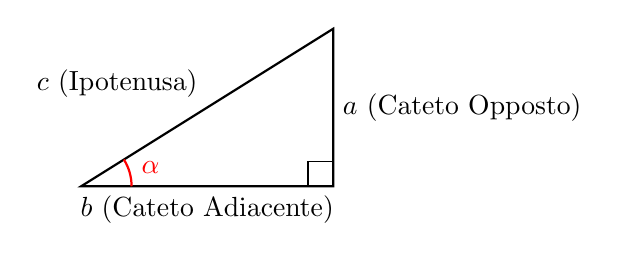
\begin{tikzpicture}[scale=0.8]
        % Triangolo
        \draw[thick] (0,0) coordinate (C) -- (4,0) coordinate (B) -- (4,2.5) coordinate (A) -- cycle;
        % Angolo retto
        \draw (3.6,0) -- (3.6,0.4) -- (4,0.4);
        % Etichette Lati
        \node[below] at (2,0) {$b$ (Cateto Adiacente)};
        \node[right] at (4,1.25) {$a$ (Cateto Opposto)};
        \node[above left] at (2,1.25) {$c$ (Ipotenusa)};
        % Angolo Alpha
        \draw[red, thick] (0.8,0) arc (0:32:0.8);
        \node[red] at (1.1,0.3) {$\alpha$};
    \end{tikzpicture}
    \end{center}
    
    \textbf{Formule Fondamentali:}
    \begin{enumerate}
        \item $\text{Cateto} = \text{Ipo} \cdot \sin(\text{opposto})$
        \[ a = c \cdot \sin \alpha \]
        
        \item $\text{Cateto} = \text{Ipo} \cdot \cos(\text{adiacente})$
        \[ b = c \cdot \cos \alpha \]
        
        \item $\text{Cateto} = \text{Altro Cateto} \cdot \tan(\text{opposto})$
        \[ a = b \cdot \tan \alpha \]
    \end{enumerate}
}
\section*{13-bis. Derivata della Funzione Inversa}

\block{
    \textbf{La Formula} \\
    Sia $y = f(x)$ una funzione invertibile. La derivata della sua inversa $f^{-1}(y)$ nel punto $y_0$ è:
    
    \[ (f^{-1})'(y_0) = \frac{1}{f'(x_0)} \]
    
    \textbf{Attenzione!} Qui $x_0$ è il punto tale che $f(x_0) = y_0$.
    \textit{Geometricamente: Le tangenti sono simmetriche rispetto alla bisettrice, quindi i coefficienti angolari sono reciproci.}
}

\block{
    \textbf{Algoritmo di Calcolo (Senza trovare l'inversa)} \\
    Se ti chiedono $(f^{-1})'(k)$, segui questi 3 step:
    
    \begin{enumerate}
        \item \textbf{TROVA LA X (Cruciale):} \\
        Risolvi l'equazione $f(x) = k$. \\
        \textit{Nota: Spesso si risolve "a occhio" provando $x=0, 1, -1, e, \pi$.}
        
        \item \textbf{DERIVA LA DIRETTA:} \\
        Calcola $f'(x)$ e sostituisci la $x$ trovata al punto 1.
        
        \item \textbf{FAI IL RECIPROCO:} \\
        Il risultato finale è $\dfrac{1}{\text{Valore trovato}}$.
    \end{enumerate}
}

\block{
    \textbf{Esempio (Classico da Esame)} \\
    Data $f(x) = x^3 + x + 2$. Calcolare $(f^{-1})'(4)$.
    
    \begin{enumerate}
        \item \textbf{Cerco x:} $x^3 + x + 2 = 4 \implies x^3+x-2=0$.
        \\ Si vede subito che $x=1$ (infatti $1+1+2=4$).
        \item \textbf{Derivo f:} $f'(x) = 3x^2 + 1$.
        \\ Valuto in $x=1$: $f'(1) = 3(1)^2 + 1 = 4$.
        \item \textbf{Reciproco:} Il risultato è $\dfrac{1}{4}$.
    \end{enumerate}
}
\newpage
\section*{15. La Funzione Integrale (Derivata)}

\block{
    \textbf{Il Teorema Fondamentale (Torricelli-Barrow)} \\
    Se $F(x) = \int_{a}^{x} f(t) \, dt$, allora $F'(x) = f(x)$.
}

\block{
    \textbf{Tabella Completa delle Derivate} \\
    \textit{Qui c'è tutto, dal caso base a quello generale.}
    
    \renewcommand{\arraystretch}{2.2} % Spazio extra per leggere bene le formule
    \begin{center}
    \begin{tabular}{|l|c|l|}
        \hline
        \textbf{Caso} & \textbf{Integrale} $F(x)$ & \textbf{Derivata} $F'(x)$ \\ \hline
        
        \textbf{Base} 
        & $\displaystyle \int_{a}^{x} f(t)dt$ 
        & $f(x)$ \\ \hline
        
        \textbf{Invertito}
        & $\displaystyle \int_{x}^{a} f(t)dt$ 
        & $-f(x)$ \\ \hline
        
        \textbf{Sopra} ($h(x)$)
        & $\displaystyle \int_{a}^{h(x)} f(t)dt$ 
        & $f(h(x)) \cdot h'(x)$ \\ \hline
        
        \textbf{Sotto} ($g(x)$)
        & $\displaystyle \int_{g(x)}^{b} f(t)dt$ 
        & $-f(g(x)) \cdot g'(x)$ \\ \hline
        
        \textbf{COMPLETO}
        & $\displaystyle \int_{g(x)}^{h(x)} f(t)dt$ 
        & $f(h(x))h'(x) \textcolor{red}{\boldsymbol{-}} f(g(x))g'(x)$ \\ \hline
    \end{tabular}
    \end{center}
    \renewcommand{\arraystretch}{1}
    
    \vspace{0.2cm}
    \textbf{Regola mnemonica per il caso Completo:} \\
    (Sostituisci \textbf{Sopra} $\times$ Derivata Sopra) \textbf{MENO} (Sostituisci \textbf{Sotto} $\times$ Derivata Sotto).
}

\block{
    \textbf{Gestire gli Infinti ($\pm \infty$)} \\
    L'infinito negli estremi si comporta come una costante: la sua derivata è 0.
    
    \[ F(x) = \int_{-\infty}^{h(x)} f(t)dt \implies F'(x) = f(h(x)) \cdot h'(x) \]
    
    \textit{Spiegazione:} Spezzi l'integrale in un punto $c$: $\int_{-\infty}^{c} + \int_{c}^{h(x)}$. La prima parte è un numero (costante), quindi derivando sparisce.
}
\section*{20. Algoritmo di Risoluzione Integrali}

\block{
    \textbf{START: Hai davanti $\int f(x) \, dx$}
    
    \begin{center}
    \textbf{1. CONTROLLO TABELLA BASE} \\
    \textit{È nella lista degli integrali fondamentali ($x^\alpha, \sin, \cos, e^x$)?}
    \end{center}
    
    \[ \downarrow \text{\textbf{NO}} \]
    
    \begin{center}
    \textbf{2. CONTROLLO GENERALIZZATI (Derivata)} \\
    \textit{Vedi una funzione $f(x)$ e FUORI la sua derivata $f'(x)$?} \\
    {\small (Es: $\int \sin^2 x \cdot \cos x \, dx$ oppure $\int \frac{2x}{x^2+1} dx$)}
    \end{center}
    
    \[ \downarrow \text{\textbf{NO}} \quad \text{(Allora analizza la STRUTTURA)} \]
    
    \renewcommand{\arraystretch}{1.5}
    \begin{center}
    \begin{tabular}{|p{0.3\linewidth}|p{0.3\linewidth}|p{0.3\linewidth}|}
        \hline
        \textbf{A. Prodotto Misto} & \textbf{B. Rapporto Polinomi} & \textbf{C. Funzioni Simili/Composte} \\ 
        \hline
        
        Hai funzioni di \textbf{famiglie diverse} moltiplicate? \newline (Es: $x \cdot e^x$, $x \cdot \ln x$) 
        & Hai una frazione con \textbf{polinomi} sopra e sotto? \newline (Es: $\frac{x+1}{x^2-4}$) 
        & Hai funzioni \textbf{della stessa famiglia} o argomenti "brutti"? \newline (Es: $\sqrt{e^x+1}$, $\cos(\sqrt{x})$) \\ 
        \hline
        
        $\downarrow$ & $\downarrow$ & $\downarrow$ \\
        
        \textbf{PER PARTI} & \textbf{FRATTI SEMPLICI} & \textbf{SOSTITUZIONE} \\ 
        (Usa LIATE) & (Scomponi e A, B) & (Poni $t = \dots$) \\ \hline
    \end{tabular}
    \end{center}
    \renewcommand{\arraystretch}{1}
    
    \vspace{0.5cm}
    \textbf{Nota sulla Sostituzione (Il Jolly):}
    Se sei bloccato e non rientri nei casi A o B, la sostituzione è l'ultima spiaggia. Cerca di porre $t$ uguale alla parte che ti dà fastidio (es: la radice, l'esponente strano, l'argomento del logaritmo).
} 
% --- INTEGRALI GENERALIZZATI ---
\section*{16. Integrali Immediati (Composti)}

\block{
    \textbf{La Regola d'Oro ($f(x)$ composta)} \\
    \textit{Se vedi una funzione "intrappolata" e fuori c'è la sua derivata, puoi integrare subito.}
    
    \[ \int g(f(x)) \cdot \textcolor{red}{f'(x)} \, dx = G(f(x)) + c \]
    
    \renewcommand{\arraystretch}{2.2}
    \begin{center}
    \begin{tabular}{|l|l|}
        \hline
        \textbf{Integrale} & \textbf{Risultato} \\ \hline
        
        $\displaystyle \int [f(x)]^n \cdot \textcolor{red}{f'(x)} \, dx$ 
        & $\dfrac{[f(x)]^{n+1}}{n+1}$ \quad {\scriptsize ($n \ne -1$)} \\ \hline
        
        $\displaystyle \int \frac{\textcolor{red}{f'(x)}}{f(x)} \, dx$ 
        & $\ln |f(x)|$ \\ \hline
        
        $\displaystyle \int e^{f(x)} \cdot \textcolor{red}{f'(x)} \, dx$ 
        & $e^{f(x)}$ \\ \hline
        
        $\displaystyle \int \sin(f(x)) \cdot \textcolor{red}{f'(x)} \, dx$ 
        & $-\cos(f(x))$ \\ \hline
        
        $\displaystyle \int \cos(f(x)) \cdot \textcolor{red}{f'(x)} \, dx$ 
        & $\sin(f(x))$ \\ \hline
        
        $\displaystyle \int \tan(f(x)) \cdot \textcolor{red}{f'(x)} \, dx$ 
        & $-\ln|\cos(f(x))|$ \\ \hline
        
        $\displaystyle \int \cot(f(x)) \cdot \textcolor{red}{f'(x)} \, dx$ 
        & $\ln|\sin(f(x))|$ \\ \hline
        
        $\displaystyle \int \frac{\textcolor{red}{f'(x)}}{\cos^2(f(x))} \, dx$ 
        & $\tan(f(x))$ \\ \hline
        
        $\displaystyle \int \frac{\textcolor{red}{f'(x)}}{\sin^2(f(x))} \, dx$ 
        & $-\cot(f(x))$ \\ \hline
        
        $\displaystyle \int \frac{\textcolor{red}{f'(x)}}{\cosh^2(f(x))} \, dx$ 
        & $\tanh(f(x))$ \quad \textcolor{orange}{(Iperbolico)} \\ \hline
        
        $\displaystyle \int \frac{\textcolor{red}{f'(x)}}{\sinh^2(f(x))} \, dx$ 
        & $-\coth(f(x))$ \quad \textcolor{orange}{(Iperbolico)} \\ \hline
        
        $\displaystyle \int \frac{\textcolor{red}{f'(x)}}{\sqrt{1-[f(x)]^2}} \, dx$ 
        & $\arcsin(f(x))$ \\ \hline
        
        $\displaystyle \int \frac{\textcolor{red}{f'(x)}}{1+[f(x)]^2} \, dx$ 
        & $\arctan(f(x))$ \\ \hline
    \end{tabular}
    \end{center}
    \renewcommand{\arraystretch}{1}
}

\block{
    \textbf{Il Caso Lineare ($ax+b$)} \\
    \textit{Se l'argomento è di primo grado, la derivata è solo la costante $a$. Bilancia dividendo fuori.}
    
    \[ \int e^{ax+b} \, dx = \frac{1}{a} e^{ax+b} \]
    \textit{Vale per tutte:} $\int \cos(3x)dx = \frac{1}{3}\sin(3x)$.
}

% --- FRATTI SEMPLICI ---
\section*{17. Fratti Semplici (Metodo dei Polinomi)}

\block{
    \textbf{Setup Iniziale} \\
    Devi calcolare $\int \frac{N(x)}{D(x)} dx$.
    \begin{enumerate}
        \item Se grado $N \ge$ grado $D$: Fai la \textbf{divisione polinomiale}.
        \item Se grado $N <$ grado $D$: Scomponi il denominatore e usa la tabella sotto.
    \end{enumerate}
}

\block{
    \textbf{I 3 Casi del Denominatore ($ax^2 + bx + c$)}
    
    \renewcommand{\arraystretch}{1.5}
    \begin{center}
    \begin{tabular}{|p{0.25\linewidth}|p{0.3\linewidth}|p{0.3\linewidth}|}
        \hline
        \textbf{Delta ($D(x)$)} & \textbf{Scomposizione} & \textbf{Struttura Somma} \\ \hline
        
        \textbf{1. $\Delta > 0$} \newline (2 radici reali distinte $x_1, x_2$) 
        & $a(x-x_1)(x-x_2)$ 
        & $\displaystyle \frac{A}{x-x_1} + \frac{B}{x-x_2}$ \newline \textit{Integrazione: Logaritmi} \\ \hline
        
        \textbf{2. $\Delta = 0$} \newline (1 radice doppia $x_1$) 
        & $a(x-x_1)^2$ 
        & $\displaystyle \frac{A}{x-x_1} + \frac{B}{(x-x_1)^2}$ \newline \textit{Occhio al quadrato sul secondo!} \\ \hline
        
        \textbf{3. $\Delta < 0$} \newline (Complesso) 
        & Irriducibile 
        & $\displaystyle \frac{Ax + B}{ax^2+bx+c}$ \newline \textit{Si risolve in 2 step (vedi sotto)} \\ \hline
    \end{tabular}
    \end{center}
    \renewcommand{\arraystretch}{1}
}

\block{
    \textbf{Come risolvere il caso $\Delta < 0$ (Il "Mostro")} \\
    L'integrale di $\frac{Ax+B}{ax^2+bx+c}$ si spezza sempre in due pezzi:
    
    \textbf{Pezzo 1: Logaritmo}
    Cerchi di far comparire la derivata del denominatore sopra (spesso moltiplicando/dividendo).
    \[ \to \ln(ax^2+bx+c) \]
    
    \textbf{Pezzo 2: Arcotangente}
    Ciò che avanza è una costante fratto il polinomio. Devi completare il quadrato al denominatore per ottenere la forma:
    \[ \int \frac{1}{1 + (\dots)^2} \to \arctan(\dots) \]
}
\section*{18. Integrazione per Parti (Metodo LIATE)}

\block{
    \textbf{1. La Formula} \\
    \[ \int f(x) \cdot g'(x) \, dx = f(x) \cdot g(x) - \int f'(x) \cdot g(x) \, dx \]
    
    Il dilemma è sempre: \textbf{Chi derivo ($f$)? Chi integro ($g'$)?}
}

\block{
    \textbf{2. La Regola LIATE (Chi derivare?)} \\
    Scegli come $f(x)$ (quella da \textbf{DERIVARE}) la funzione che compare \textbf{PRIMA} in questa lista. L'altra sarà $g'(x)$ (da integrare).
    
    \begin{center}
    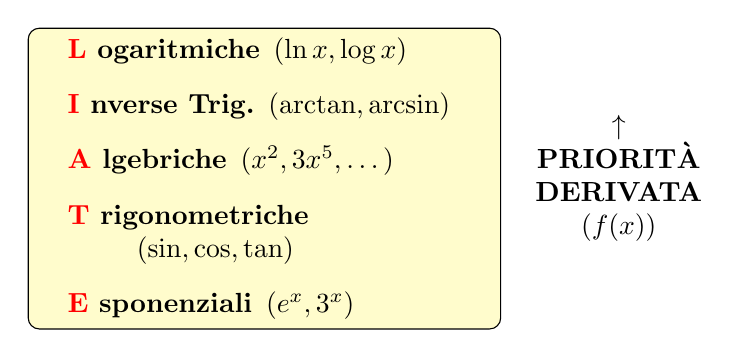
\begin{tikzpicture}
        \node[fill=yellow!20, draw, rounded corners, minimum width=6cm] (box) {
        \begin{minipage}{5cm}
            \begin{description}
                \item[\textcolor{red}{L} \text{ogaritmiche}] ($\ln x, \log x$)
                \item[\textcolor{red}{I} \text{nverse Trig.}] ($\arctan, \arcsin$)
                \item[\textcolor{red}{A} \text{lgebriche}] ($x^2, 3x^5, \dots$)
                \item[\textcolor{red}{T} \text{rigonometriche}] ($\sin, \cos, \tan$)
                \item[\textcolor{red}{E} \text{sponenziali}] ($e^x, 3^x$)
            \end{description}
        \end{minipage}
        };
        \node[right of=box, xshift=3.5cm, text width=2.5cm, align=center] {
            $\uparrow$ \\ \textbf{PRIORITÀ} \\ \textbf{DERIVATA} \\ ($f(x)$)
        };
    \end{tikzpicture}
    \end{center}
    
    \textbf{Esempi:}
    \begin{itemize}
        \item $\int x \cdot \ln x \, dx$: Ho \textbf{A} ($x$) e \textbf{L} ($\ln$).
        \\ La \textbf{L} vince su A. $\to$ Derivo $\ln x$, integro $x$.
        \item $\int x \cdot e^x \, dx$: Ho \textbf{A} ($x$) e \textbf{E} ($e^x$).
        \\ La \textbf{A} vince su E. $\to$ Derivo $x$, integro $e^x$.
    \end{itemize}
}

\block{
    \textbf{3. Il Caso Speciale "Ciclico" (Boomerang)} \\
    Se hai \textbf{E}sponenziale + \textbf{T}rigonometrica (es: $\int e^x \sin x dx$), sono in fondo alla lista insieme.
    \begin{enumerate}
        \item Applica la formula due volte.
        \item Tornerai all'integrale di partenza (con un segno o coefficiente diverso).
        \item Portalo a sinistra dell'uguale e somma.
    \end{enumerate}
    \[ I = \dots - I \implies 2I = \dots \implies I = \frac{1}{2}(\dots) \]
}
\section*{19. Algebra e Proprietà Fondamentali}

\block{
    \textbf{1. Proprietà dei Logaritmi (Salva-Derivate)} \\
    \textit{Usale PRIMA di derivare per evitare calcoli mostruosi.}
    
    Siano $A, B > 0$:
    \begin{itemize}
        \item \textbf{Prodotto $\to$ Somma:}
        \[ \ln(A \cdot B) = \ln A + \ln B \]
        
        \item \textbf{Rapporto $\to$ Differenza:}
        \[ \ln\left(\frac{A}{B}\right) = \ln A - \ln B \]
        \textit{Utile per spezzare frazioni giganti nello studio di funzione.}
        
        \item \textbf{Esponente $\to$ Moltiplicazione (VITALE):}
        \[ \ln(A^k) = k \cdot \ln A \]
        \textit{Esempio:} Derivare $\ln(x^{50})$ è difficile. Scrivi $50 \ln x$ e la derivata è immediata ($50/x$).
        
        \item \textbf{Cambio Base:} $\log_a x = \frac{\ln x}{\ln a}$
    \end{itemize}
    \textbf{Nota:} $\ln(1) = 0$, $\ln(e) = 1$.
}

\block{
    \textbf{2. Proprietà delle Potenze}
    \begin{itemize}
        \item $x^a \cdot x^b = x^{a+b}$ \quad (Sommi esponenti)
        \item $(x^a)^b = x^{a \cdot b}$ \quad (Moltiplichi esponenti)
        \item $\frac{1}{x^a} = x^{-a}$ \quad (Giri la frazione)
        \item $\sqrt[b]{x^a} = x^{\frac{a}{b}}$ \quad (Radice $\to$ Esponente fratto)
    \end{itemize}
}

\block{
    \textbf{3. Prodotti Notevoli (Da sapere a memoria)}
    
    \textbf{Quadrato di Binomio:}
    \[ (A \pm B)^2 = A^2 \pm 2AB + B^2 \]
    
    \textbf{Cubo di Binomio:}
    \[ (A + B)^3 = A^3 + 3A^2B + 3AB^2 + B^3 \]
    \[ (A - B)^3 = A^3 - 3A^2B + 3AB^2 - B^3 \]
    \textit{Mnemonica: 1, 3, 3, 1. Se c'è il meno, i segni si alternano (+ - + -).}
    
    \textbf{Differenza di Quadrati:}
    \[ A^2 - B^2 = (A-B)(A+B) \]
    
    \textbf{Somma/Differenza di Cubi:}
    \[ A^3 - B^3 = (A-B)(A^2 + AB + B^2) \]
    \[ A^3 + B^3 = (A+B)(A^2 - AB + B^2) \]
    \textit{Nota: La seconda parentesi è un "Falso Quadrato" (non ha il 2 nel mezzo) ed è sempre irriducibile ($\Delta < 0$).}
}

\end{document}